\documentclass[a4paper,12pt]{article}
\pdfoutput=1 
\usepackage{jheppub}
\usepackage[T1]{fontenc} % if needed
\usepackage{tabularx}
\usepackage{graphicx}
\usepackage[utf8]{inputenc}
\usepackage{isomath}


\title{\boldmath Constraints on Beyond Standard Model vector boson interactions 
		in an effective field theory using differential cross section of the production 
		of two jets associate with four charged leptons at 
		$\sqrt{s} = 13$ TeV with the ATLAS detector}
		\author{Dong Qichen}
		\affiliation{The University of Manchester,\\316 Oxford Road, UK}
		\emailAdd{dong.qichen@student.manchester.ac.uk}
		\abstract{In this report, the production of a pair on-shell Z bosons 
		associate with a pair of jets in an electroweak enhanced phase space region 
		was measured at centre-of-mass energy $\sqrt{s} = 13$ TeV with $139\ fb^{-1}$ 
		of pp collision data collected by the ATLAS detector. The result is compatible with
		the Standard Model prediction.
		The differential cross sections as functions of two CP-sensitive observables were
		obtained by removing the detector effect from the measurement. The differential 
		measurements were then reinterpreted in a dimension-6 Standard 
		Model Effect Field Theory and constraints on relevent CP-odd and CP-even new 
		physics operators were obtained.}


\begin{document} 
	\maketitle
	\flushbottom

	\section{Introduction}
		\label{sec:intro}
		\par The Standard Model of particle physics (SM)\cite{Gaillard_1999} has been
		a very successful theory in predicting the nature of fundamental particles and their interactions.
		However, the SM is not yet complete, for example, the enormous matter-antimatter asymmetry\cite{Canetti_2012}
		observed in the universe is not fully described by the SM. Being sensitive to Beyond the SM (BSM)
		physics is one of the main goals of the Large Hadron Collider (LHC)\cite{Evans_2008}. At current energy 
		scale, the BSM effects may manifest themselves as small corrections to the SM, searching for 
		deviations from the SM prediction; therefore a general way to search the new physics phenomena.

		\par Since the discovery of the last particle predicted by the SM, the Higgs boson, in 2012\cite{Aad_2012}, 
		the nature of its interactions with other particles has been carefully investigated in order 
		to seek any deviations from the SM. The Vector Boson Scattering (VBS) process\cite{rauch2016vectorboson}, 
		an important pure electroweak process in the LHC, enables us to probe the nature of Higgs 
		boson interactions with vector bosons and to constrain BSM hypothesis altering the nature of the 
		Higgs boson and vector bosons which may provide alternative Electroweak Symmetry Breaking (EWSB) 
		mechanism\cite{dawson1999introduction} and additional sources of CP violation\cite{peccei1995cp}.

		\par In the LHC, VBS events are produced by a pair of vector bosons 
		radiated from the colliding partons scattered to another pair of 
		vector bosons subsequently. At the detector-level, the signature 
		of VBS events are two jets from the initial partons associate 
		with the decay products of two vector boson, and we denote such 
		events VVjj. The evidence of electroweak production of ${W^{\pm}W^{\pm}jj}$
		(EW ${W^{\pm}W^{\pm}jj}$) was first observed during the 
		first run of LHC with the ATLAS detector\cite{Aad_2014}; and the observation of this very process has been 
		confirmed by the CMS\cite{Chatrchyan:2008aa} collaboration during the second 
		run of LHC in 2018\cite{Sirunyan_2018}, while the observation in the EW ZZjj channel 
		was reported in 2019\cite{ATLAS-CONF-2019-033}. In spite the endeavour 
		has been put on the VBS process, the model-independent measurement of the differential 
		cross section has not been made so far.

		\par With a total of $139\ fb^{-1}$ proton proton collision data at 
		$\sqrt{s} = 13$ TeV acummulated in the ATLAS detector\cite{Aad:2008zzm} 
		during the second run of the LHC, a great opportunity to scrutinise the SM at 
		much higher accuracy has been provided. In this report, the fiducial differential cross section 
		of ZZjj process measured at $\sqrt{s} = 13$ TeV using the whole run II data is reported and 
		the results has been used to constrain a BSM effective field theory\cite{Brivio_2017} which provides 
		alternative Higgs boson interactions, vector boson interactions and additional source of CP violation 
		in the electroweak sector.

	\section{Recap} \label{sec:recap}
		\par In the last semester\cite{last:2020}, an iterative unfolding procedure to remove the detector effect\cite{DAgostini:1994fjx} 
		was performed on the data corresponding to an integrated luminosity of $36\ fb^{-1}$ using the 
		ATLAS detector in a VBS enhanced fiducial phase space. Three distributions which are possibly sensitive to the 
		BSM physics effect were unfolded, namely $\Delta\phi_{jj}$, $M_{jj}$ and $M_{4l}$, detailed discussion on
		these observables can be found in Ref. \cite{last:2020}. The unfolding procedure also gives the covariance
		matrices which take the bin to bin migration into account. With these infrastructures  in hand, the differential 
		cross section in various distributions can be easily measured; and the constraints on BSM physics theories can be set using the covariance matrices
		and the corresponding differential cross section, the detail of which will be discussed in section \ref{ss:lsp}.
	\section{ZZjj differential cross section} \label{sec:xsmea}
		\subsection{ZZjj processes and backgrounds}
			\par The ATLAS detector in the LHC is a layered designed general-purpose particle detector, the technical detail of which 
			can be found in Ref. \cite{Aad:2008zzm}. The detector signatures of VVjj events in the ATLAS detector have a variety of 
			patterns, which depend on the kind of final state vector bosons, namely $W$ or $Z$ boson; and the decay channel 
			of them\cite{Watkins:1986va}. ZZjj events with both Z bosons decay leptonically are denoted ZZjj4l, which is the selected
			channel in this analysis. Although the branching ratio for both Z bosons decay leptonically is around $10^{-3}$\cite{PhysRevD.98.030001},
			the channel has the minimal hadronic background and no missing momenta.

			\par At the leading order, the ZZjj4l events can be separated to two categories, the electroweak production with six
			electroweak vertices (EW\ ZZjj4l), and the QCD production including two strong-interaction vertices and four electroweak
			vertices (QCD\ ZZjj4l), at the current energy scale, the QCD\ ZZjj4l production has a cross section approximately 100 
			times larger than the cross section of EW production, which is around 1 fb. The QCD\ ZZjj4l can be further separated by the
			initial species of initial partons. If both initial partons are gluon, the process is classified as ggZZ4l, 
			otherwise classified as qqZZ4l. Some example leading order Feynman diagrams of these processes are shown in figure \ref{fig:feynman}.
			\begin{figure}[ht]
				\begin{centering}
				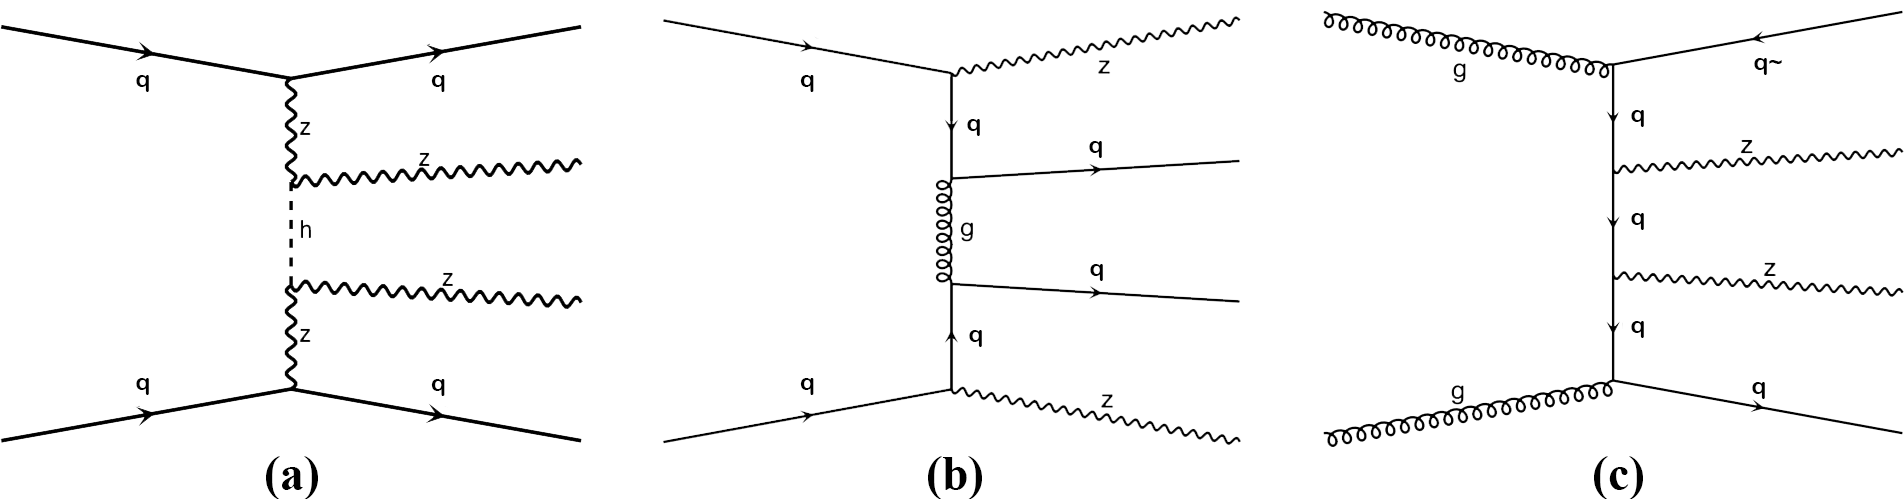
\includegraphics[scale=0.42]{figures/feynman.png}
				\caption{The leading order SM Feynman diagrams contributing to ZZjj processes. \textbf{(a)} EW\ ZZjj process, \textbf{(b)} QCD\ qqZZjj process and \textbf{(c)} is QCD\ ggZZjj process.}
				\label{fig:feynman}
				\end{centering}
			\end{figure}
			\par In addition to the large QCD\ ZZjj background, other non-ZZjj processes may produce the same or similar final states as the VBS processes; 
			these background processes, therefore, mimic the detector signature of VBS process. non-ZZjj background processes  
			considered in this analysis are the production of one vector boson plus a Higgs boson, the Higgs boson then decays to four
			charged leptons (VH4l); the production of three vector bosons (VVV); and the production of two charged leptons and a 
			pair of $t\bar{t}$ quarks (ttll),  the decay of the top quark via W bosons give birth to another pair of charged leptons. 
			All three backgrounds are order six pure EW processes at leading order, which is the same order as VBS process. The 
			example Feynman diagrams of these background processes at leading order are shown in figure \ref{fig:feynman_bkg}. 
			Contribution of other processes in the studied phase space were neglected. 
			\begin{figure}[ht]
				\begin{centering}
				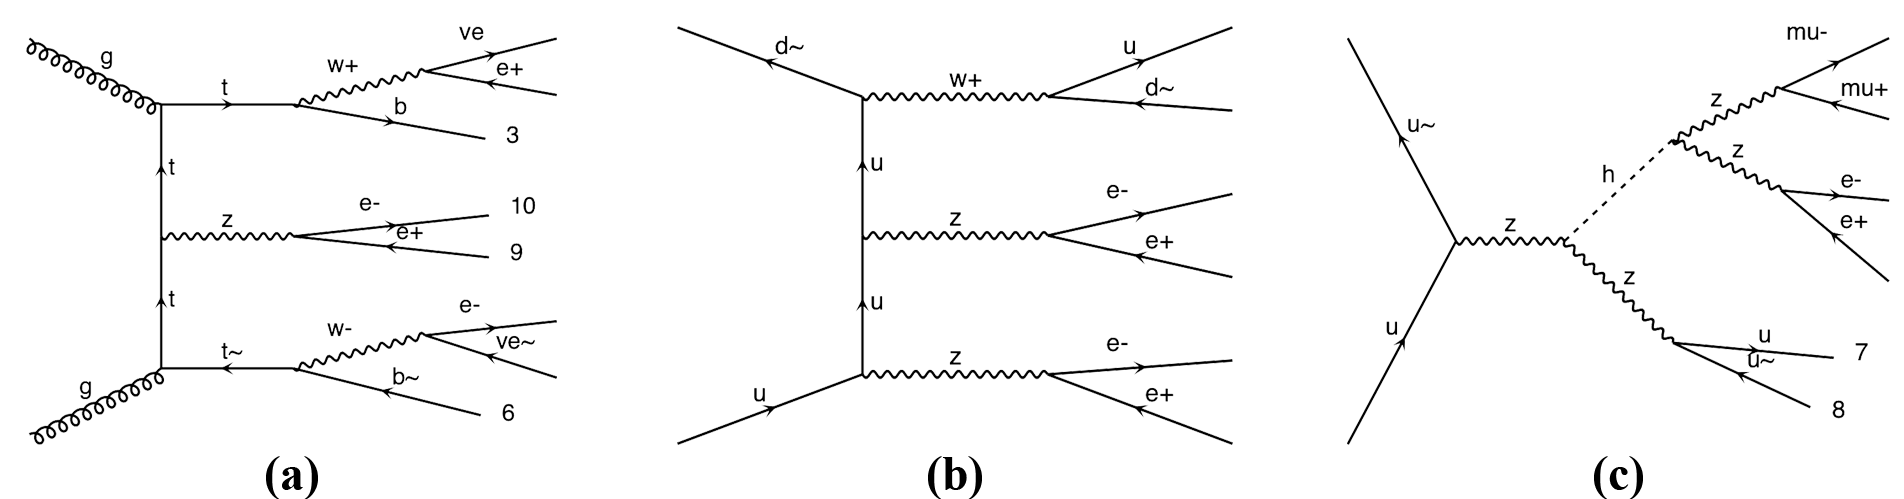
\includegraphics[scale=0.42]{figures/feynman_bkg.png}
				\caption{The leading order SM feynman diagrams contributing to non-ZZjj background processes, 
				subsequent decay of the intermediate particles are also shown. 
				\textbf{(a)} ttll process, \textbf{(b)} ZZ$W^{+}$ process and \textbf{(c)} ZH process.}
				\label{fig:feynman_bkg}
				\end{centering}
			\end{figure}
			\par Despite the extreme rarity and enormous background of EW\ ZZjj4l process, there exist region in the phase 
			space where the EW\ ZZjj4l is enhanced while other background processes are suppressed. With $36 fb^{-1}$ of data,
			the significance of the EW\ ZZjj4l process was measured to be $1.5\sigma$. The detailed discussion can be found
			in the first-semester report\cite{last:2020}. 
		\subsection{Data and Simulations}
			\par This analysis was performed using the proton-proton collision data recorded in the ATLAS detector 
			during the run II of LHC with centre-of-mass energy $\sqrt{s} = 13\ TeV$. These events were required 
			to pass the online trigger system\cite{zurNedden:2238679}, which has an overall efficiency of 96\% 
			to 99\%\cite{Aaboud_2019}. The total accumulated data sample corresponding to an integrated luminosity 
			of $139\ fb^{-1}$ was used in this analysis.
			
			\par Monte Carlo (MC) Simulated events\cite{10.5555/3172929} are used in this analysis to correct the 
			detector-level events for detector effects, and to estimate the expected contribution of signal and 
			background processes. The ATLAS collaboration has switched to a newer version of software to generate 
			MC simulations, which gives better Next-to-Leading-Order (NLO) estimations and updated jets reconstruction
			algorithm compared to MC simulations used last semester\cite{last:2020}.

			\par The EW\ ZZjj4l process with no on-shell Higgs boson intermediate state was modelled by the 
			\textsc{Sherpa 2.2.2}\cite{Freeman_2001} event generator with NNPDF3.0NNLO Parton Distribution Functions (PDF)\cite{Ball_2015} at 
			leading order (LO), parton showering was handled by the \textsc{Sherpa CSShower}\cite{Bothmann_2019}. The Higgs EW\ ZZjj4l, in other 
			word Vector Boson Fusion (VBF), events were simulated at NLO precision in QCD using 
			\textsc{Powheg-Box}\cite{Oleari_2010} interfaced to \textsc{Pythia 8}\cite{Sj_strand_2015} , detailed NLO correction 
			of the VBF process can be found in Ref. \cite{Nason_2010}.
			For $gg \rightarrow H\rightarrow ZZ\rightarrow4l$ events, \textsc{Powheg-Box} event generator and similar NLO 
			precision QCD estimation\cite{Alioli:2008tz} were chosen. Other $ggZZ4l$ processes were modelled using \textsc{Sherpa 2.2.2}
			with NNPDF3.0NNLO PDF at LO; the results were merged with \textsc{CSShower} parton showering.
			The QCD qqZZ4l events were also modelled separately, $t\bar{t}\rightarrow H\rightarrow ZZ\rightarrow 4l$ events were generated
			at NLO\cite{Hartanto:2015uka} using \textsc{Powheg-Box}, while other qqZZ4l events were modelled by \textsc{Sherpa 2.2.2} generator
			with NNPDF3.0NNLO PDF at LO, and \textsc{CSShower} parton showering was used to model hadronization of final-state quarks.
			The VH background events were generated at NLO precision with MiNLO\cite{Hamilton_2012} using \textsc{Powheg-Box} event 
			generator with NNPDF3.0 PDF and \textsc{Pythia 8} showering.
			The VVV and ttll processes were modelled by \textsc{Sherpa 2.2.2} with NNPDF3.0NNLO PDF at LO.

			\par Each particle-level MC simulation event goes through detailed ATLAS detector simulation\cite{Aad_2010} based on
			the \textsc{Geant 4}\cite{AGOSTINELLI2003250} framework to produce detector-level simulation events. The detector simulation of Every 
			process gives three ``generations'' of simulation files, each generation corresponds to a specific detector status, neighbouring 
			bunch crossings (pile-up), integrated luminosity in one year of operation of the LHC.

		\subsection{Events selection}\label{ss:selection}
			\begin{table}[ht]
				\centering
				\renewcommand\arraystretch{1.1}
				\begin{tabularx}{\textwidth}{X c} 
					\hline\hline
					Object 				& 		fiducial region \\
					\hline
					Electrons 			& 		\begin{tabular}{c} ``Loose'' ID criterion\\ ``FixedCutPflowLoose'' criterion\\$p_T > 7$ GeV, $|\eta| < 2.47$ \\ $|d_0/\sigma_{d_0}| < 5,\  |z_0 \times sin\theta| < 0.5$ mm \end{tabular} \\
					\hline 
					Muons 				& 		\begin{tabular}{c} ``Loose'' ID criterion\\ ``FixedCutPflowLoose'' criterion\\$p_T > 7 \text{\ GeV},\ |\eta| < 2.7$ \\ $|d_0/\sigma_{d_0}| < 3,\  |z_0 \times \text{sin}\theta| < 0.5 \text{mm}$\end{tabular} \\
					\hline
					Jets 				& 		\begin{tabular}{c}$P_T > 30$ GeV and $Jvt > 0.6$ for $|\eta| < 2.4$ \\ $P_T > 40$ GeV for $2.4< |\eta| < 4.5$\end{tabular} \\
					\hline
					OCSF lepton pairs 	& 		\begin{tabular}{c} two pairs of OCSF lepton with $M_Z$ closest to Z mass \\ $p_T > 20, 20, 10$ GeV for leading 3 leptons \\ $\Delta{R_{l^+l^-}} > 0.2$ \\$70\ \text{GeV}<M_{Z} < 110$ GeV \end{tabular} \\
					\hline
					Dijets system 		& 		\begin{tabular}{c}leading two jets with $y_{j_1} \times y_{j_2} < 0$ and $|y_{j_1} - y_{j_2}| > 2$\\ dijet invariant mass $M_{jj} > 200$ GeV\end{tabular} \\
					\hline 
					ZZjj system  		&		$P_{T}\ balance < 0.5$\\
					\hline\hline
				\end{tabularx}
				\caption{Summary of selections applied to simulated and observaed events.}
				\label{tab:cut}
			\end{table}
			\par The selection of ZZjj4l events relies on the final state particles of the ZZjj4l processes, 
			namely electrons, muons and jets. All the selections discussed here were implimented using the \textsc{Cern Root} framework\cite{ANTCHEVA20092499}.
			\par Electrons were identified by the energy deposit in the electromagnetic calorimeter with corresponding 
			tracks in the inner tracking detector (ID). Muons were reconstructed by the tracks in the muon spectrometer (MS)
			matched to tracks in the ID, muons can also be identified by the MS alone in the region where the ID does not cover.
			Jets are clustered by the energy deposit in the hadronic calorimeter using the particle flow (PFlow)\cite{Aaboud_2017} 
			algorithm.

			\par The selecting criteria are mostly unchanged from last semester,
			which can be found in Ref. \cite{last:2020}, the only differences are that last semester one of the 
			Z boson can be off-shell, this time the mass of the second pair of Opposite Charge, Same Flavour (OCSF) lepton 
			pair was required to have an invariant mass above 70 GeV, which means both Z bosons are on-shell Z boson, and a 
			jet vertex tagger (Jvt)\cite{Kehinde_2017} was applied to jets with $|\eta| < 2.4$ this semester to select jets 
			with higher possibility come from hard interactions. The selection requirements applied are summarised in T
			able \ref{tab:cut}, definitions of abbreviations and symbols can be found in Ref. \cite{last:2020}.
			
			\par Both the predicted particle-level and detector-level SM events were required to satisfy
			all criteria listed above, apart from selections that not appliable to particle-level events, for example,
			the lepton ID criterion and Jvt selection. The real-world data events were required to pass the same 
			selections as well. The selection of the BSM EFT particle-level events was implemented using the 
			\textsc{Rivet}\cite{Bierlich_2020} framework and the jets reconstruction algorithm chosen was $anti-k_t$\cite{Cacciari_2008} 
			with radius parameter $R=0.4$; other criteria were the same as the SM particle-level selections.
			\par The observed and SM predicted event yields in the fiducial region are listed in Table \ref{tab:fidyield}, where the
			``Other'' row denotes the overall contribution of $VVV$, $VH$ and $ttll$ processes.
			The observed event yield shows no significant deviation from the SM prediction. The significance of EW ZZjj process 
			is measured to be $2.18\sigma$, which corresponds to a p-value $= 8.7\times10^{-4}$. Some selections, for example, 
			$M_{jj}$ were deliberately raised or abolished compared to the last semester\cite{last:2020} to let more QCD 
			ZZjj events into the fiducial region, which is essential for BSM physics models limit setting, 
			details will be discussed in section \ref{ss:lsp}.
			\begin{table}[ht]
				\centering
				\renewcommand{\arraystretch}{1.1}
				\begin{tabularx}{0.5\textwidth}{X r} 
					\hline\hline
					Process 	& 		Events yield \\
					\hline
					EW ZZjj4l   & 		$22.9\pm 0.1$ \\				
					QCD qqZZ4l	&		$101.3\pm 0.5$ \\
					QCD ggZZ4l  & 		$26.9\pm 0.2$ \\
					Other 		& 		$7.9\pm 0.1$ \\
					\hline
					Total		&		$158.9\pm 0.6$\\
					\hline		
					Data		&		$164$ \\
					\hline\hline
				\end{tabularx}
				\caption{The SM predicted and observed ficucial event yields for studied processes. Uncertainties 
				quoted are statistical only.}
				\label{tab:fidyield}
			\end{table}
		\subsection{Chosen Observables} \label{ss:observables}
			\par To be sensitive to the CP-odd BSM physics model, the distributions of observables selected should be 
			sensitive to CP-violating effects; in this analysis, several CP-sensitive observables have been investigated.
			\par The most potent observable in probing CP-violation is the signed azimuthal angle between the leading and 
			subleading jets\cite{Bernlochner_2019},
			\begin{equation}\label{eq:dpjj}
				\Delta\phi_{jj} = \phi_{1} - \phi_{2}
			\end{equation}
			where the ordering of jets is determined by the rapidity of them so that $j_1$ is the jet with higher rapidity
			(more forward in space). By artificially selecting one direction, the $\Delta\phi_{jj}$ is by definition sensitive to 
			the Parity violation\cite{PhysRev.105.1413}.
			The other chosen observable, $theta_1$\cite{Bolognesi_2012}, is defined as the angle between the leading Z boson and the third lepton 
			measured in the ZZ rest frame, i.e.
			\begin{equation}\label{eq:the1}\theta_1 = \text{cos}^{-1}(\frac{\mathbfit{Z_1\cdot l_3}}{\mathbfit{|\mathbf{Z_1}||\mathbfit{l_3}|}})\end{equation}
			where the bold character denotes the three-vector of particles in ZZ rest frame. Other observables mentioned 
			in Ref. \cite{Bolognesi_2012} were investigated as well, but $\theta_1$ was chosen for its best 
			sensitivity to the CP-even BSM EFT operators, more on that in section \ref{ss:lsp}.
			\par These distributions were initially finely binned and later re-binned to variable bin sizes, the bin width 
			were determined by requiring at least 14 expected detector-level ZZjj events each bin. The expected and observed detector-level 
			event yields as functions of the two selected observables are shown in figure \ref{fig:Evtyields}. The observation is compatible 
			with the SM predictions.
			\begin{figure}[ht]
				\begin{centering}
				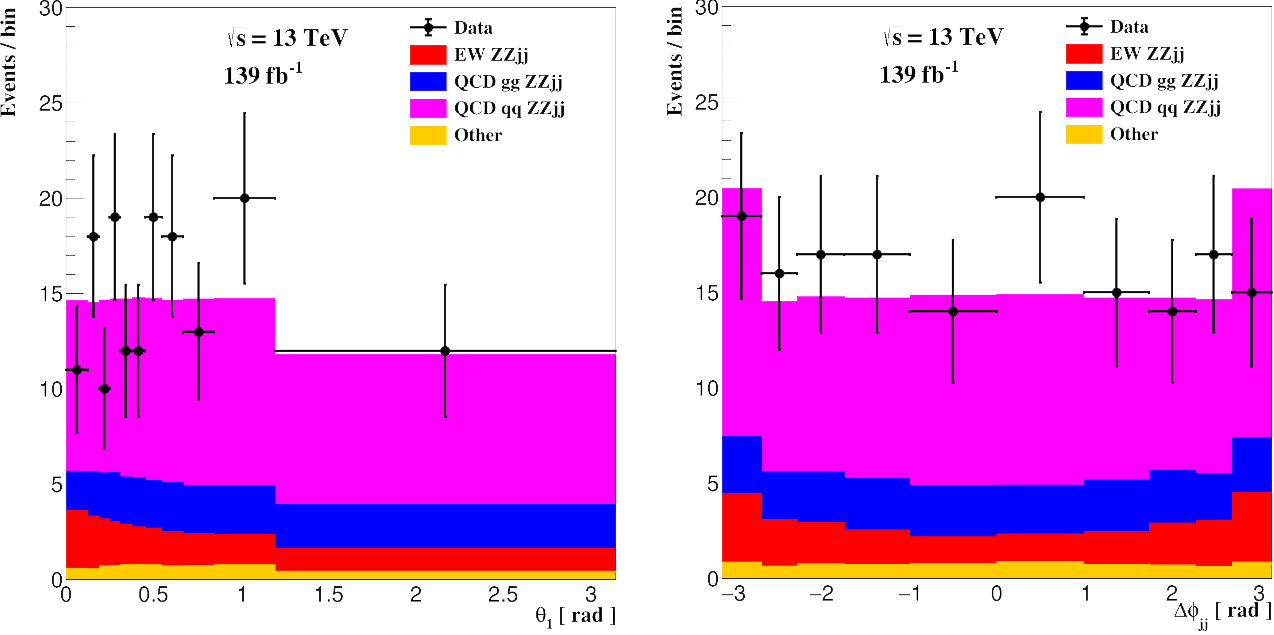
\includegraphics[scale=0.673]{figures/binyields.png}
				\caption{The observed and expected event yield as function of $\theta_1$ and $\Delta\phi_{jj}$ with variable bin width.}
				\label{fig:Evtyields}
				\end{centering}
			\end{figure}
		\subsection{Unfolding}
			\par The measured $\Delta\phi_{jj}$ and $\theta_1$ spectra were unfolded to remove detector effects, including
			the efficiency of the trigger system, and limited resolution and efficiency of the tracking detectors and calorimeters\cite{Schmitt_2017}.
			The unfolding procedure also gives the covariance matrices account for the correlation between bins in a given distribution.
			By performing such correction, the results become model-independent so that they can be directly compared with 
			BSM particle-level predictions. 
			\par The unfolding procedure relies on the thorough understanding of the ATLAS detector, in other words, how would
			particle-level final-state particles interact with the detector and what detector-level signals are expected.
			The imperfection of the detector results in events migration, fake signals and missing particles. Since the direct access to particle-level 
			events is impossible, those three effects are estimated by the particle-level and detector-level simulations and represented by 
			a respond matrix $R_{ij}$; more details can be found in Ref. \cite{last:2020}. An iterative unfolding algorithm\cite{DAgostini:1994fjx} 
			using the particle-level predicted distributions as an initial hypothesis, implemented by RooUnfold framework\cite{adye2011unfolding} was used 
			to achieve the unfolding. One iteration was found to be a good balance between bias and statistical uncertainties for both distributions.
			\par Before the unfolding procedure, the non-ZZjj background contributions were removed from the observed data, leaving only ZZjj 
			contributions; the faked events were then removed, and the iterative method was performed; finally, a bin-by-bin efficiency correction 
			was applied. 
		\subsection{Results}
			\par After applying the unfolding technique, the event yields can be easily be reinterpreted to the differential cross section
			in the fiducial region. The measured and expected fiducial differential cross section as functions of selected observables are shown in figure \ref{fig:diffxs}, showing no significant deviation from the SM predictions
			\begin{figure}[ht]
				\begin{centering}
				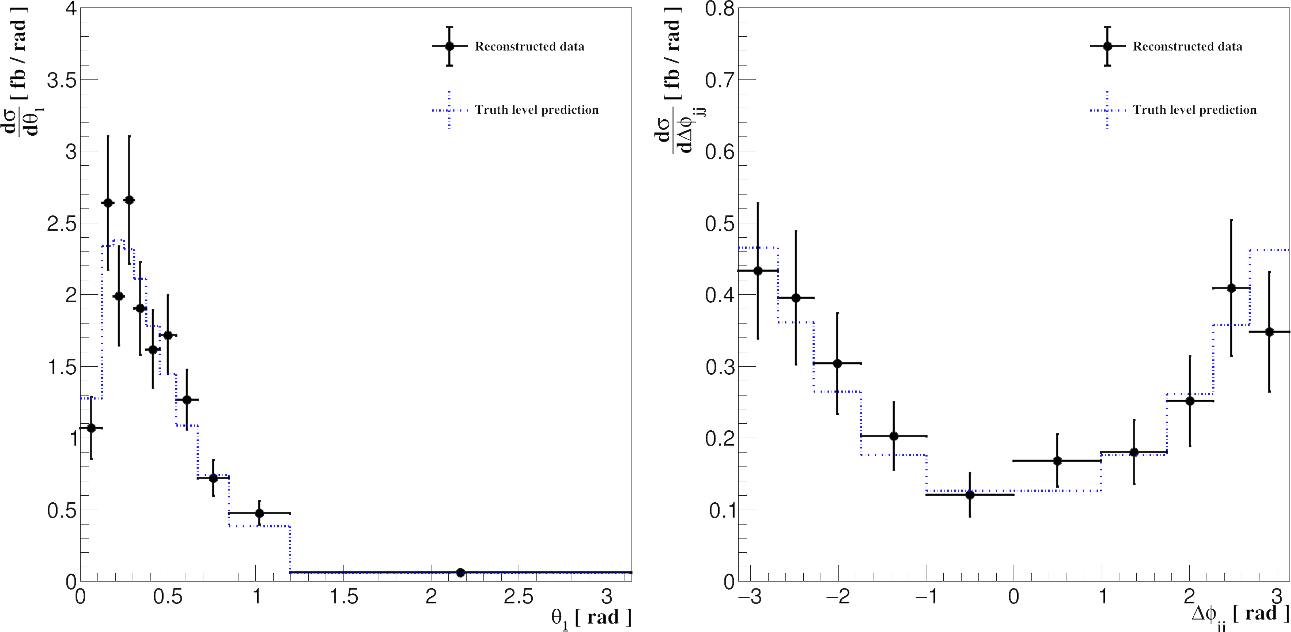
\includegraphics[scale=0.664]{figures/diffxs.png}
				\caption{The observed and expected fiducial cross sections as functions of $\theta_1$ and $\Delta\phi_{jj}$.}
				\label{fig:diffxs}
				\end{centering}
			\end{figure}
	\section{Reinterpretation in an effective field theory} \label{sec:eft}
		\subsection{EFT theory}
			\par In the SM, no CP-violation is predicted in the electroweak interactions; however, as stated, the SM is incomplete. 
            In the SMEFT, the SM is treated as a low-energy (infrared) leading order approximation of a yet to be determined grand theory when 
            new physics phenomena reside in a much higher energy scale, in this case, $\Lambda >> \bar{v}_T$. One can expend 
            the SM by constructing a series of expansion in the order of the ratio to new physics scale. With the SM Lagrangian defined in Ref. \cite{Salam:1968rm}, the
            EFT Lagrangian constructed using $SU(3)\times SU(2)\times U(1)$ symmetry with dimension-6 BSM operators can be written as 
			\begin{equation}\label{eq:lagr}
				\mathcal{L}_{EFT} = \mathcal{L}_{SM} + \mathcal{L}^{(6)},\ \ \ \mathcal{L}^{(6)} = \sum_{i}\frac{c_i}{\Lambda^2}\mathcal{O}
			\end{equation} 
			where $c_i$ is the Wilson coefficient, and $\mathcal{O}_i$ is the corresponding dimension-6 BSM operator, higher dimensional Lagrangian
			was neglected. The structure of the Lagrangian allows us to split the quantum amplitude, square of matrix element, to the SM and BSM part, i.e.
			\begin{equation}\label{eq:amp}
				|\mathcal{M}|^2 = |\mathcal{M}_{SM}|^2 + 2\text{Re}(\mathcal{M}_{SM}^\dagger\mathcal{M}_{EFT}) + |\mathcal{M}_{EFT}|^2 + \mathcal{O}(\Lambda^{-6})
			\end{equation}
			where $2\text{Re}(\mathcal{M}_{SM}^\dagger\mathcal{M}_{EFT})$ is proportional to $\Lambda^{-2}$, which corresponds to the interference 
			between the SM and EFT, and $|\mathcal{M}_{EFT}|^2$ is proportional to $\Lambda^{-4}$, which is the direct EFT contribution. 
			In this report, only one BSM operator is discussed at a time, so we hereby denote the cross 
			section corresponding to each component of the amplitude. The total cross section can be written as
			\begin{equation}\label{eq:eftxs}
			\sigma_{EFT}(C) = \sigma_{SM} + \frac{C}{\Lambda^{2}}\sigma_{Linear} + \frac{C^2}{\Lambda^{4}}\sigma_{Quad}
			\end{equation} 
			where the $Quad$ and $Linear$ indicate the corresponding cross section are proportional to $c^2$ and $c$ respectively.

			\par The VBS process typically contains VVV, HVV and Vqq interaction vertices, EFT operators provide alternative interactions to these 
			vertices, for example, by exchanging unknown massive fermion whose mass is much higher than the Higgs boson. Studied EFT operators 
			are summarised in Table \ref{tab:EFTcoe}, in which the $\psi$ is the Higgs field, $W$ and $B$ are the $SU(3)\times SU(2)\times U(1)$ electroweak field tensor  and $\tau^I$ is the generator 
			of the $SU(2)$ symmetry group. The operators with $\tilde{W}^I_{\mu\nu} = \epsilon^{IJK}W^{JK}_{\mu\nu}/2$ provide 
			CP-violating effect trough the interference with the SM, while the operators without tilde are CP-even.
			For CP-odd operators, the integrated $\sigma_{Linear}$ vanish\cite{Azatov_2017} so that can only be probed by CP-sensitive 
			observables, whereas the $\sigma_{Quad}$ can be probed by the total cross section deviation from the SM prediction.
			\begin{table}[ht!]
				\centering
				\renewcommand{\arraystretch}{1.1}
				\begin{tabularx}{0.75\textwidth}{X l r} 
				\hline\hline
				Coefficient  		& Operator 																	& Relevent vertices\\
				\hline
				$c_W$               & $\epsilon^{IJK}W_\mu^{I,\nu}W_{\nu}^{J,\rho}W_{\rho}^{K,\mu}$ 			& VVV\\
				$c_{\tilde{W}}$     & $\epsilon^{IJK}\tilde{W}_\mu^{I,\nu}W_{\nu}^{J,\rho}W_{\rho}^{K,\mu}$ 	& VVV\\
				\hline
				$c_{HW}$            & ${\psi^\dagger}{\psi}W_{\mu\nu}^IW^{I,\mu\nu}$ 							& HVV\\
				$c_{H\tilde{W}}$    & ${\psi^\dagger}{\psi}\tilde{W}_{\mu\nu}^IW^{I,\mu\nu}$ 					& HVV\\
				\hline
				$c_{HWB}$           & ${\psi^\dagger}\tau^I{\psi}W_{\mu\nu}^IB^{\mu\nu}$ 						& HVV and Vqq\\
				$c_{H\tilde{W}B}$   & ${\psi^\dagger}\tau^I{\psi}\tilde{W}_{\mu\nu}^IB^{\mu\nu}$ 				& HVV and Vqq\\           
				\hline\hline
				\end{tabularx}
				\caption{Studied Wilson coefficients and corresponding EFT operators, the interaction vertices they altered are also listed.}
				\label{tab:EFTcoe}
			\end{table}

		\subsection{particle-level EFT event generation}
			\par The parton-level EW ZZjj EFT events were generated at centre-of-mass energy of 13 TeV using \textsc{Madgraph 5}\cite{Alwall_2014} event generator,
			with the SMEFTsim\cite{Brivio_2017} EFT implementation. The chosen SMEFTsim package is a simplified $U(3)^5$ EFT model
			which dramatically reduces the number of Wilson coefficients (69\cite{Brivio_2017} versus 2499 for full SMEFT\cite{Alonso_2014}) 
			thus reduces the need for computation power. The $\{M_W, M_Z, G_F\}$ input scheme was chosen for certain theoretical 
			advantages and better precision over the $\{\alpha_{EW}, M_Z, G_F\}$ input scheme\cite{Brivio_2017}.
			The parton-level results were then passed to \textsc{Pythia 8}\cite{Sj_strand_2015}
			to model the decay of Z boson and the hadronization of final-state quarks. The particle-level events then go
			through the same selections described in section \ref{ss:selection}. The EFT events the selections were reimplemented using
			the \textsc{Rivet} framework\cite{Bierlich_2020}.
			\par The linear and quadratic EFT events of EW jj4l process were generated separately with only one Wilson 
			coefficient set to $c=5$, while others set to zero, and the scale factor was set to $\Lambda=1$ TeV. One 
			can scale the resulting spectra using the proportional rule for $\sigma_{Linear}$ and $\sigma_{Quad}$, see 
			equation \ref{eq:eftxs}, to get distributions corresponding to other values of the Wilson coefficient.
			
			\par Due to the limitation of computing resources, I am not able to generate adequate EW jj4l events to minimise
			the statistical fluctuation. As a result, only processes with two on-shell Z bosons were generated to 
			keep generating time reasonable. The predicted SM differential cross-sections as a function of $\Delta\phi_{jj}$ 
			generated with and without the off-shell Z boson in the fiducial region are shown in figure \ref{fig:SMvali}, indicating
			little difference between the two samples in the fiducial region. 
			\begin{figure}[ht]
				\begin{centering}
				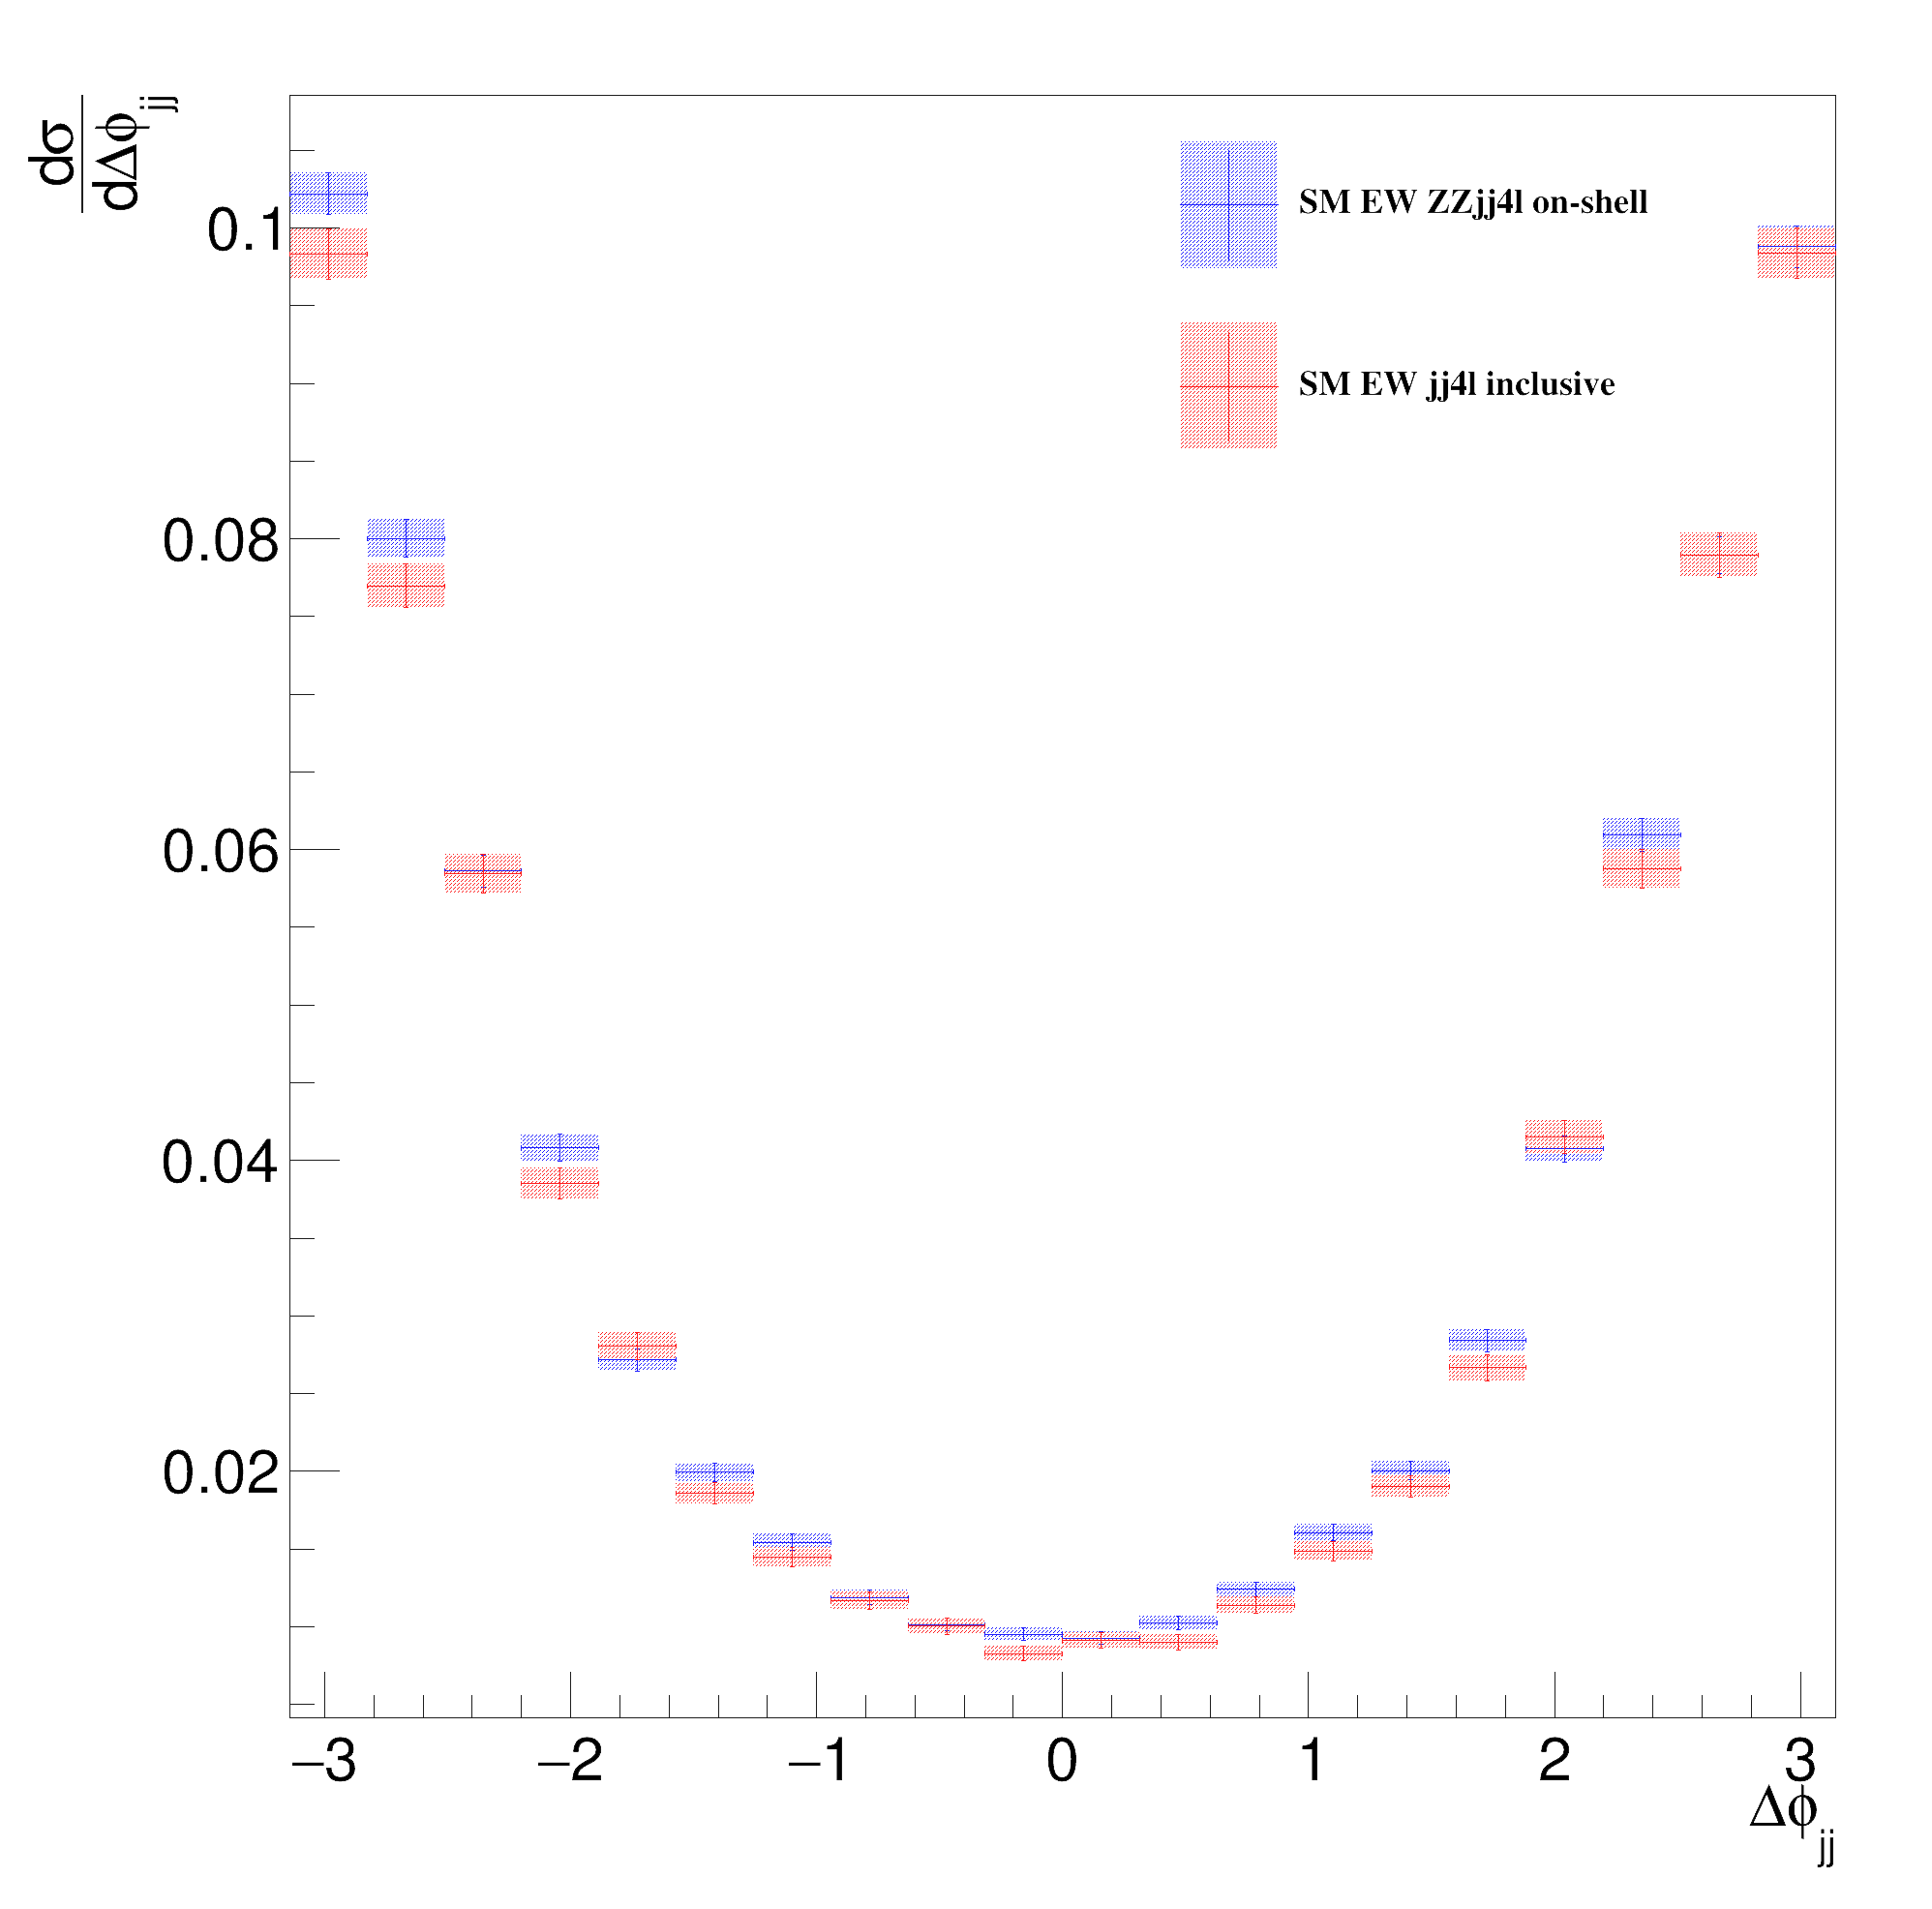
\includegraphics[scale=0.15]{figures/smvali.png}
				\caption{The predicted SM differential cross-section as function of $\Delta\phi_{jj}$ generated with and without the off-shell Z boson in the fiducial region, indicating no obvious mismodelling by not generating processes with off-shell Z bosons.}
				\label{fig:SMvali}
				\end{centering}
			\end{figure}
			\par In figure \ref{fig:EFToverSMph} and \ref{fig:EFToverSMth}, the ratio of EFT differential cross sections with $C=1$ as functions of 
			$\Delta\phi_{jj}$ and $\theta_1$ to the SM prediction are shown. the $\Delta\phi_{jj}$ spectrum shows excellent sensitivity to the 
			CP-odd EFT operators, and $\theta_1$ spectrum shows great sensitivity to CP-even EFT operators. The most considerable EFT effect is 
			the contributions corresponding to Wilson coefficients $C_W$ and $C_{\tilde{W}}$, while little sensitivities were shown for
			$C_{HWB}$ and $C_{H\tilde{W}B}$. To quantify the inclusive CP-violation, a geometrical asymmetry $A$ is defined as
			\begin{equation}
				A = \frac{\sigma_{+} - \sigma_{-}}{\sigma_{+} + \sigma_{-}}
			\end{equation}
			
			where $\sigma_{\pm}$ is the cross section in the positive and negative $\Delta\phi_{jj}$ part in the fiducial
			region. The change of fiducial cross sections and induced Asymmetries by each EFT operator with $C=1$ are summarised in Table \ref{tab:EFTeff},
			indicating the CP-odd operators do not affect the total cross section at linear order but do have contributions to the Asymmetry.
			Note that at $C=1$ the quadratic contributions are similar to the linear contributions, at larger Wilson coefficient
			the quadratic correction can dominate the EFT effect.
			\begin{figure}[ht]
				\begin{centering}
				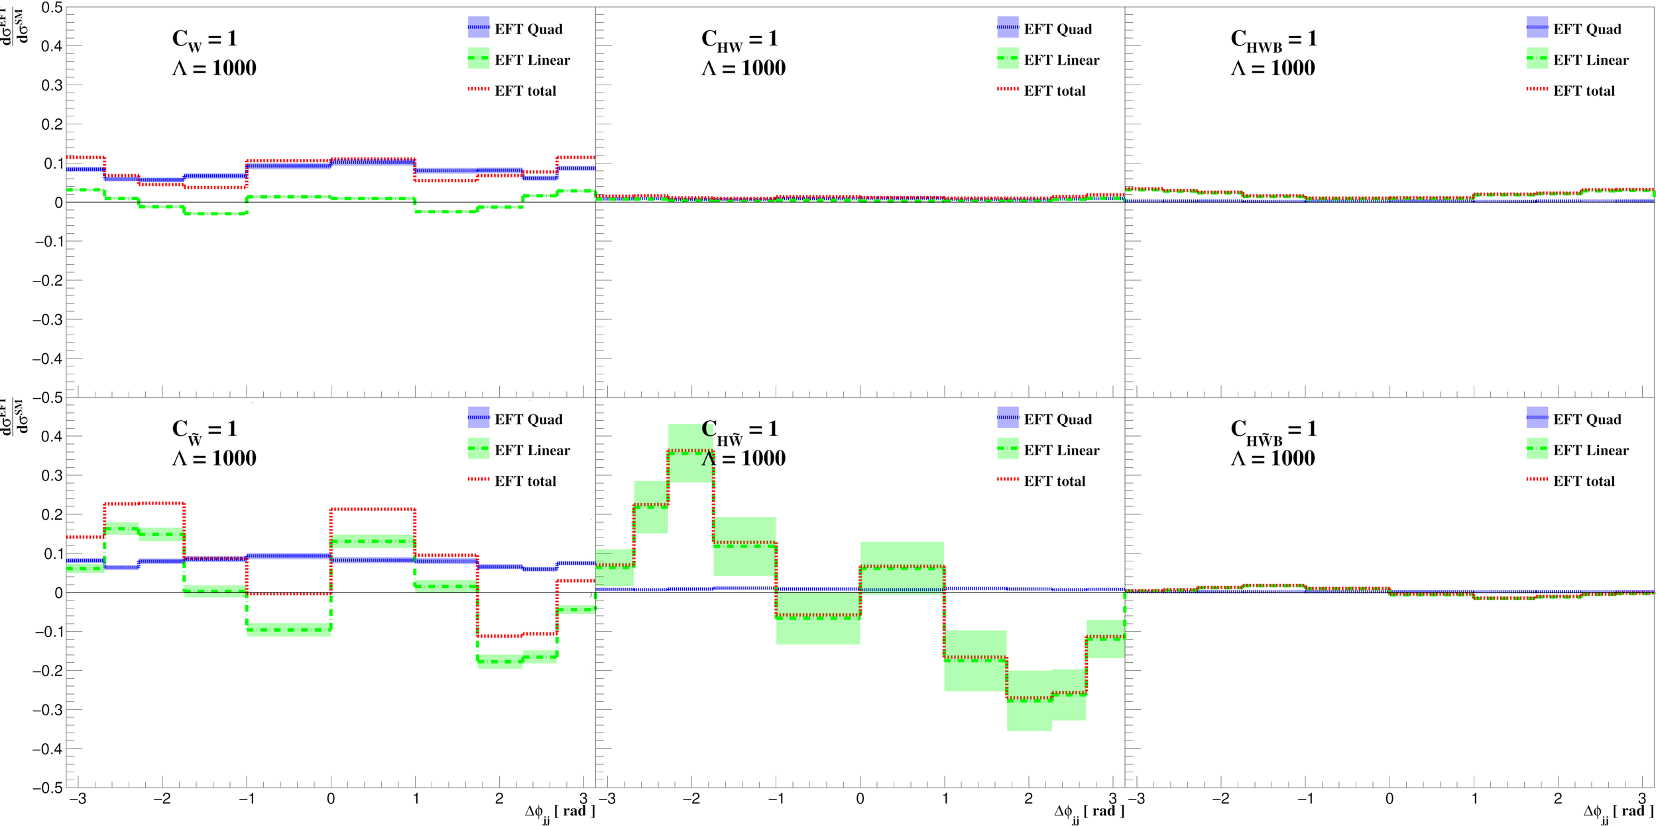
\includegraphics[scale=0.515]{figures/eftoversmphi.png}
				\caption{The ratio of EFT differential cross section with $C=1$ as function of $\Delta\phi_{jj}$ to the SM predicted cross sections, showing that the $\Delta\phi_{jj}$ spectrum have great sensitivity to CP-odd EFT operators.}
				\label{fig:EFToverSMph}
				\end{centering}
			\end{figure}
			\begin{figure}[ht]
				\begin{centering}
				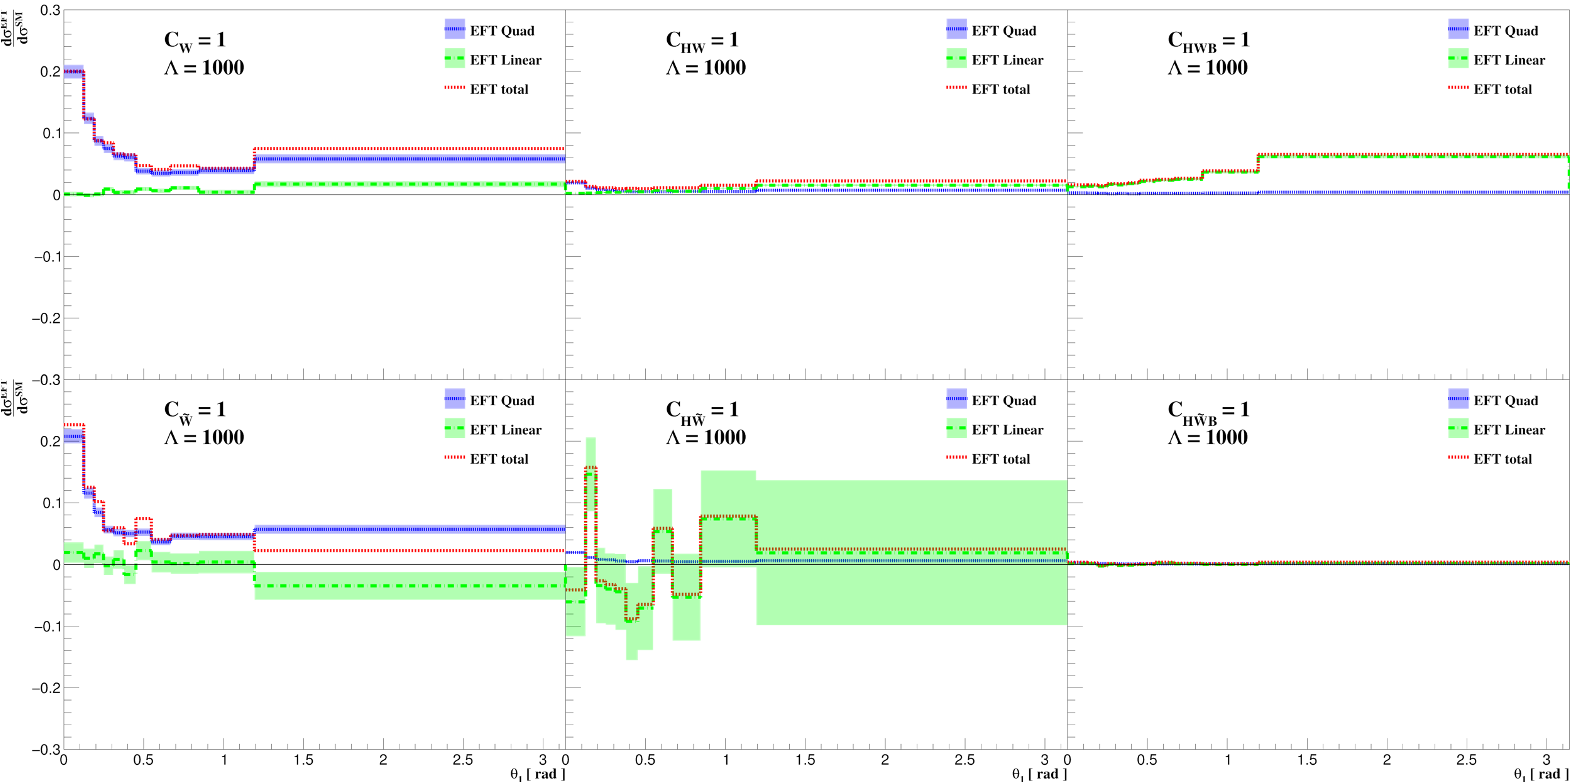
\includegraphics[scale=0.54]{figures/eftoversmthe.png}
				\caption{The ratio of EFT differential cross section with $C=1$ as function of $\theta_1$ to the SM predicted cross sections, showing that the $\theta_1$ spectrum have great sensitivity to CP-even EFT operators.}
				\label{fig:EFToverSMth}
				\end{centering}
			\end{figure}

			\begin{table}[ht!]
				\centering
				\renewcommand{\arraystretch}{1.2}
				\begin{tabularx}{\textwidth}{l c c c c} 
				\hline\hline
				Type  		& $\sigma_{Linear}$ [fb] 				& $\sigma_{Quad}$ [fb]  		& $\sigma_{EFT}/\sigma_{SM}$		& Asymmetry \\
				\hline
				SM					& -						 		& - 			  				& -									& $0.002\pm 0.003$\\
				\hline
				$c_W$               &  $0.008\pm0.002$			 	& $0.119\pm0.004$				& $0.082\pm0.003$					& $0.003\pm0.003$\\
				$c_{\tilde{W}}$     &  $0.006\pm0.008$				& $0.117\pm0.004$				& $0.080\pm0.006$					& $-0.059\pm0.006$\\
				\hline
				$c_{HW}$            &  $0.0083\pm0.0005$			& $0.0117\pm0.0003$				& $0.0130\pm0.0004$					& $-0.002\pm0.003$\\
				$c_{H\tilde{W}}$    &  $-0.02\pm0.03$ 				& $0.0117\pm0.0003$				& $-0.00\pm0.02$					& $-0.15\pm0.02$\\
				\hline
				$c_{HWB}$           &  $0.0342\pm0.0008$ 		 	& $0.00313\pm0.00007$			& $0.0242\pm0.0005$					& $-0.002\pm0.003$\\
				$c_{H\tilde{W}B}$   &  $0.0002\pm0.0007$ 			& $0.00175\pm0.00004$			& $0.0012\pm0.0005$					& $-0.010\pm0.003$\\           
				\hline\hline
				\end{tabularx}
				\caption{The predicted EFT fiducial cross section, their ratio to the SM prediction and the Asymmetries at $C=1$ and $\Lambda=1$ TeV. The uncertainties
				quoted are statistical only.}
				\label{tab:EFTeff}
			\end{table}
		\subsection{Limit setting procedure} \label{ss:lsp}
			\par With relatively high observed statistics in each bin of the two studied distributions, the uncertainties
			can be modelled by Gaussian. The $\chi^2$ function constructed to set limits on the Wilson coefficients is defined as
			\begin{equation}\label{eq:chi2}
				\chi^2 = (\overrightarrow{\sigma}_{data} - \overrightarrow{\sigma}_{EFT})^T\textbf{Cov}^{-1}(\overrightarrow{\sigma}_{data} - \overrightarrow{\sigma}_{EFT})
			\end{equation}
			where $\overrightarrow{\sigma}_{data}$ and $\overrightarrow{\sigma}_{EFT}$ are the vectors of observed and predicted EFT cross sections in every bin of a particular distribution, 
			$\textbf{Cov}$ is the statistical covariance matrix given by the the unfolding procedure. Each time two of the Wilson coefficients $C_1$, $C_2$ was scaned and a pair of $\{C_1^{min}, C_2^{min}\}$ which minimise the 
			$\chi^2$ was determined. The $\Delta\chi^2$ was constructed by 
			\begin{equation}\label{eq:Dchi2}
				\Delta\chi^2(C_1, C_2) = \chi^2(C_1, C_2) - \chi^2_{min}
			\end{equation}
			According to the Wilk's theorem\cite{wilks1938}, the $\Delta\chi^2$ also follows the $\chi^2$ distribution, whose 
			corresponding Number of Degrees of Freedom (NDF) equals the remaining free parameters, in this case, 2.
			The Confidence Level (CL) of each point on the plane was calculated by 
			\begin{equation}
				1-CL = \int^{\infty}_{\Delta\chi^2}{f_{k=2}(x)dx}
			\end{equation}
			where the $\chi^2_{min}$ is the minimum $\chi^2$ on the plane and $f_k(x)$ is the $\chi^2$ 
			distribution function with NDF $k=2$. 
		\subsection{Results}
			\par The 68\% and 95\% expected and observed limits on two of the studied CP-odd Wilson coefficients with 
			other coefficients set to 0 calculated using the $\Delta\phi_{jj}$ distribution are 
			shown in the left panel right panels in Figure \ref{fig:LimitCt}, the asymmetries on the plane are also overlayed. 
			The observed $\Delta\chi^2$ are shown in the left panels. 
			\par The 68\% and 95\% expected and observed limits on two of the studied CP-even Wilson coefficients with 
			other coefficients set to 0 calculated using the $\theta_1$ distribution are 
			shown in the left panel right panels in Figures \ref{fig:LimitC}.
			The observed $\Delta\chi^2$ are shown in the left panels. 
			\par The one-dimensional observed and expected constraints of individual Wilson coefficient are also calculated, 
			in this case the NDF of the $\Delta\chi^2$ distribution was set to 1 
			so that the resulting limits are quite tighter than the two-dimensional limits. The results are summarised in Table \ref{tab:limit}.
			As expected, the $\Delta\phi_{jj}$ distribution is more sensitive to CP-odd operators, whereas the $\theta_1$ distribution gives 
			tighter limits on CP-even Wilson coefficients.

		\begin{figure}[ht]
			\begin{centering}
			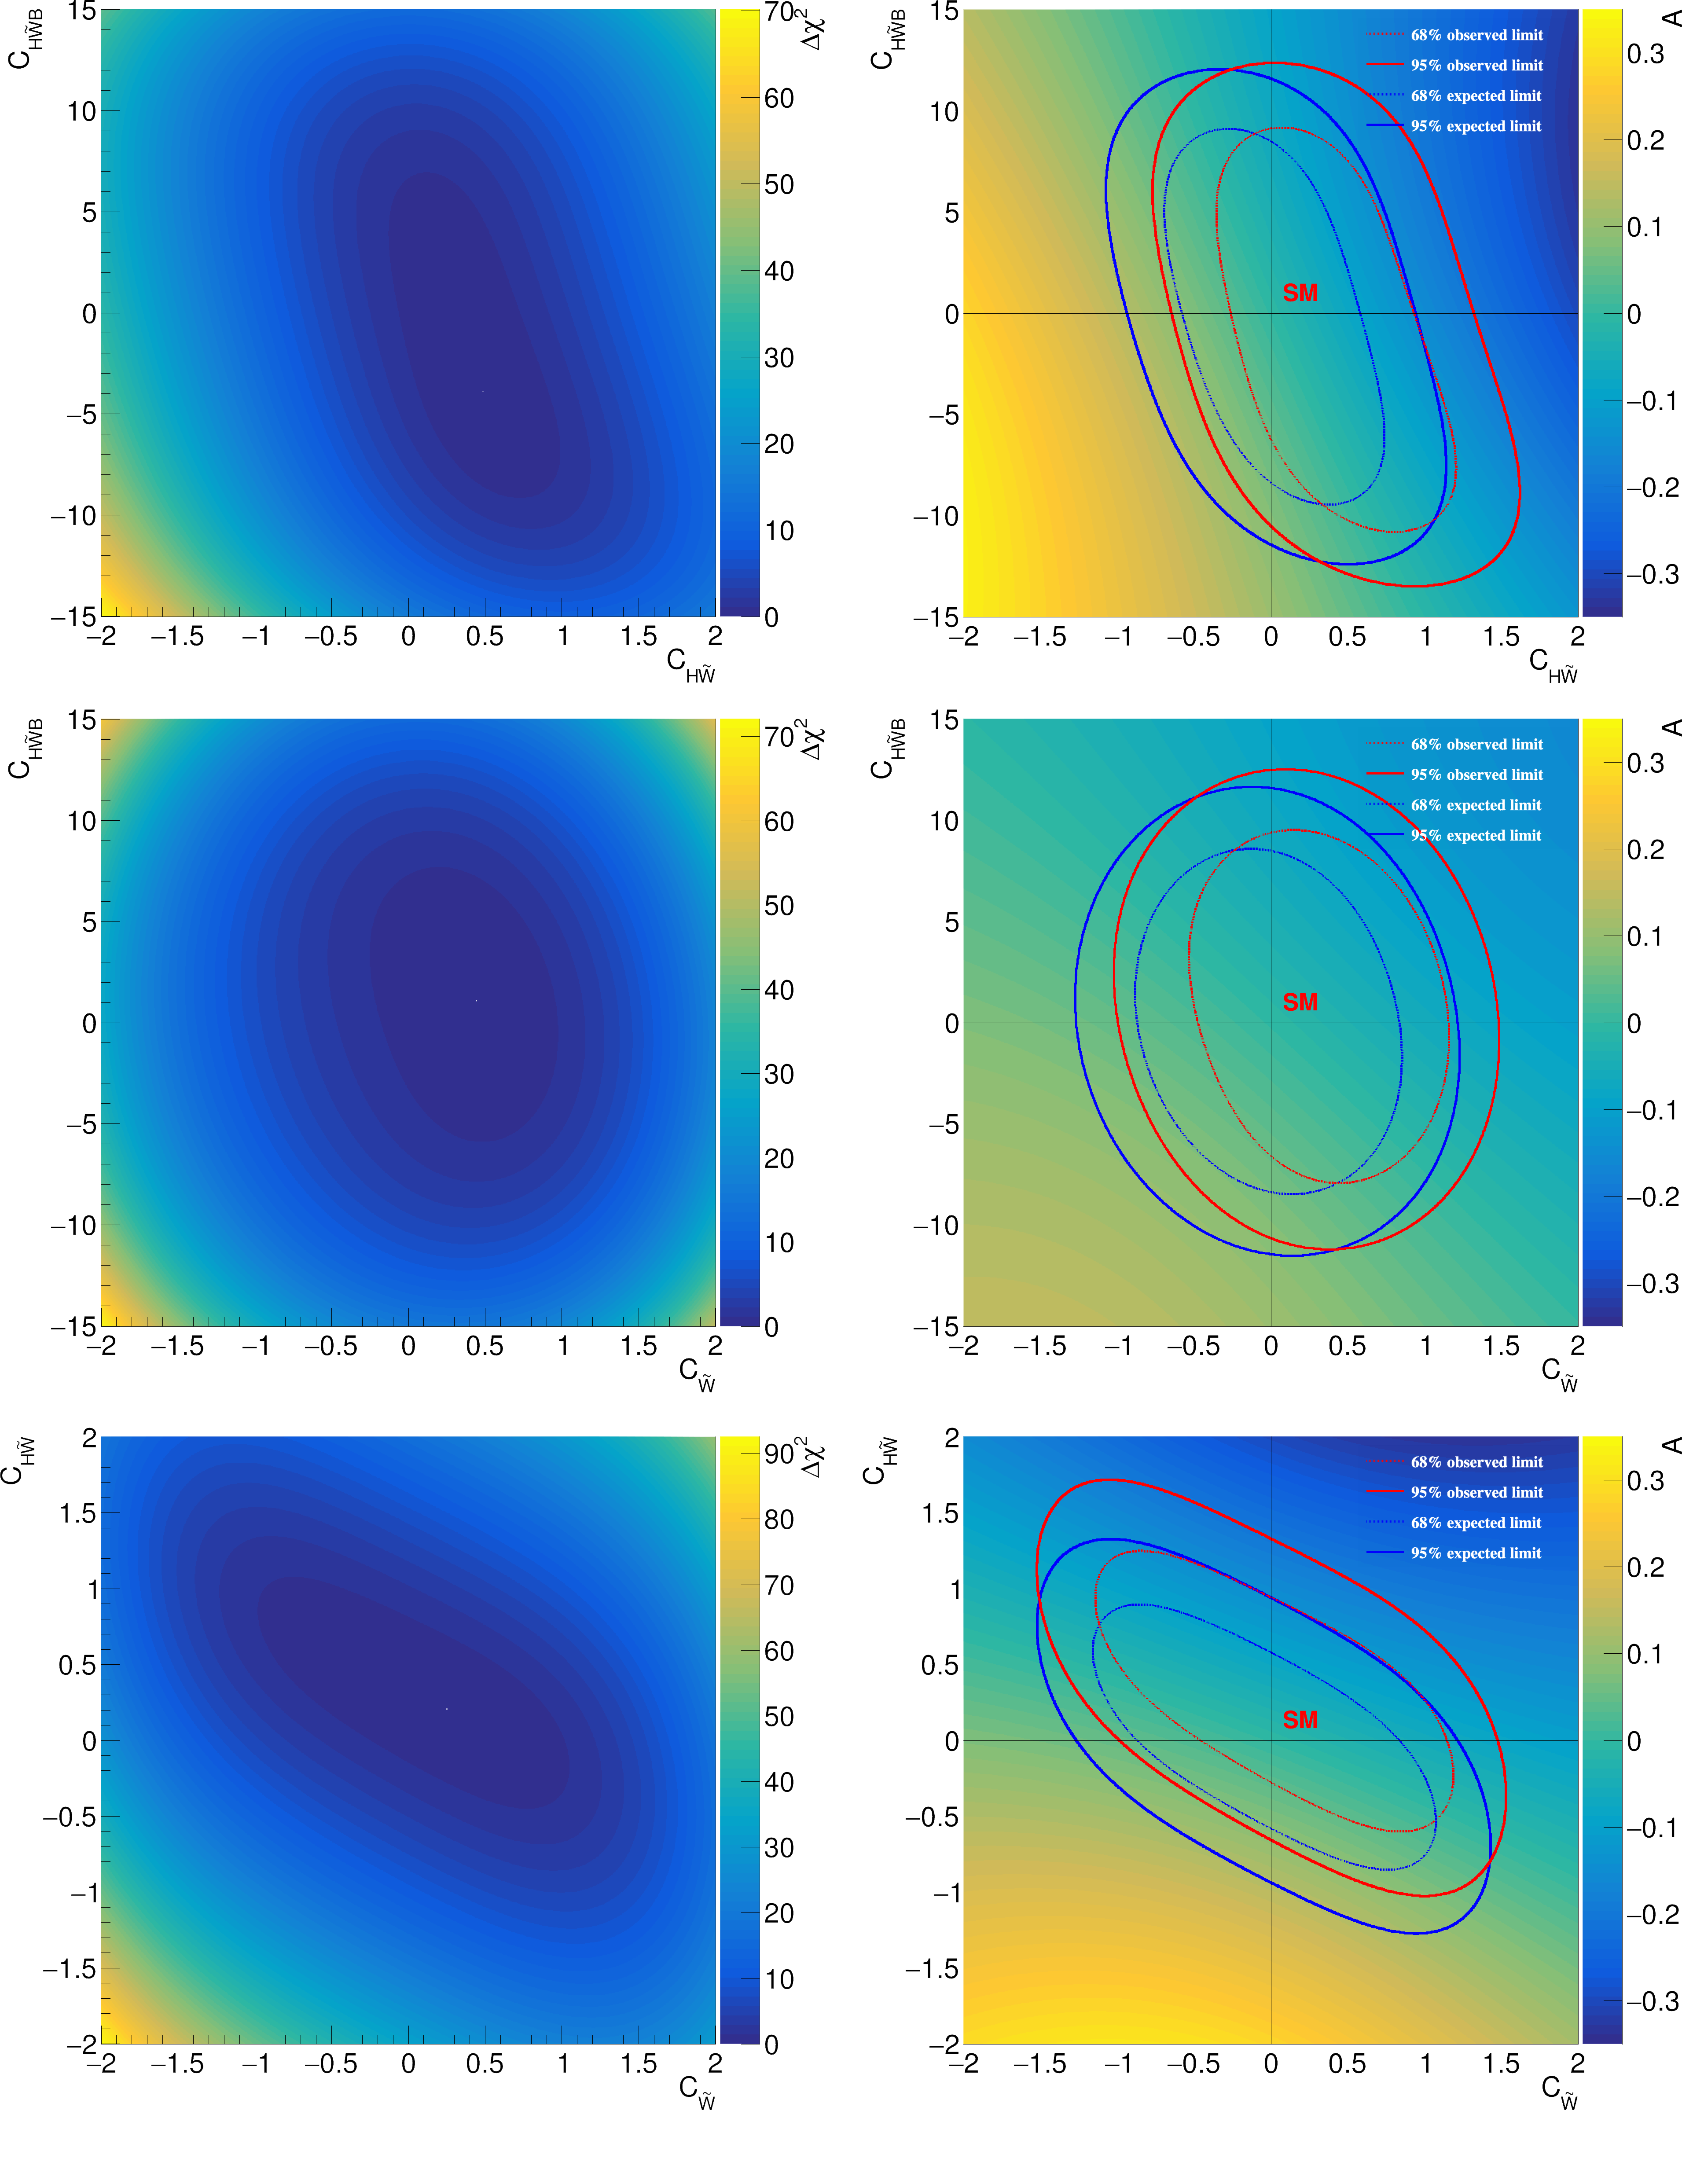
\includegraphics[scale=0.1122]{figures/limitCt.png}
			\caption{\textbf{(Left)} The $\Delta\chi^2$ calculated using the $\Delta\phi_{jj}$ distribution on the plane where 2 CP-odd Wilson coefficients were scanned 
					 \textbf{(Right)} 68\% and 95\% expected and observed limits on two of the studied CP-odd Wilson coefficients with asymmetries overlayed.
					 From top to bottom there are the $C_{H\tilde{W}}$ and $C_{H\tilde{W}B}$ plane,  $C_{\tilde{W}}$ and $C_{H\tilde{W}B}$ plane and $C_{\tilde{W}}$ and $C_{H\tilde{W}}$ plane.}
			\label{fig:LimitCt}
			\end{centering}
		\end{figure}

		\begin{figure}[ht]
			\begin{centering}
			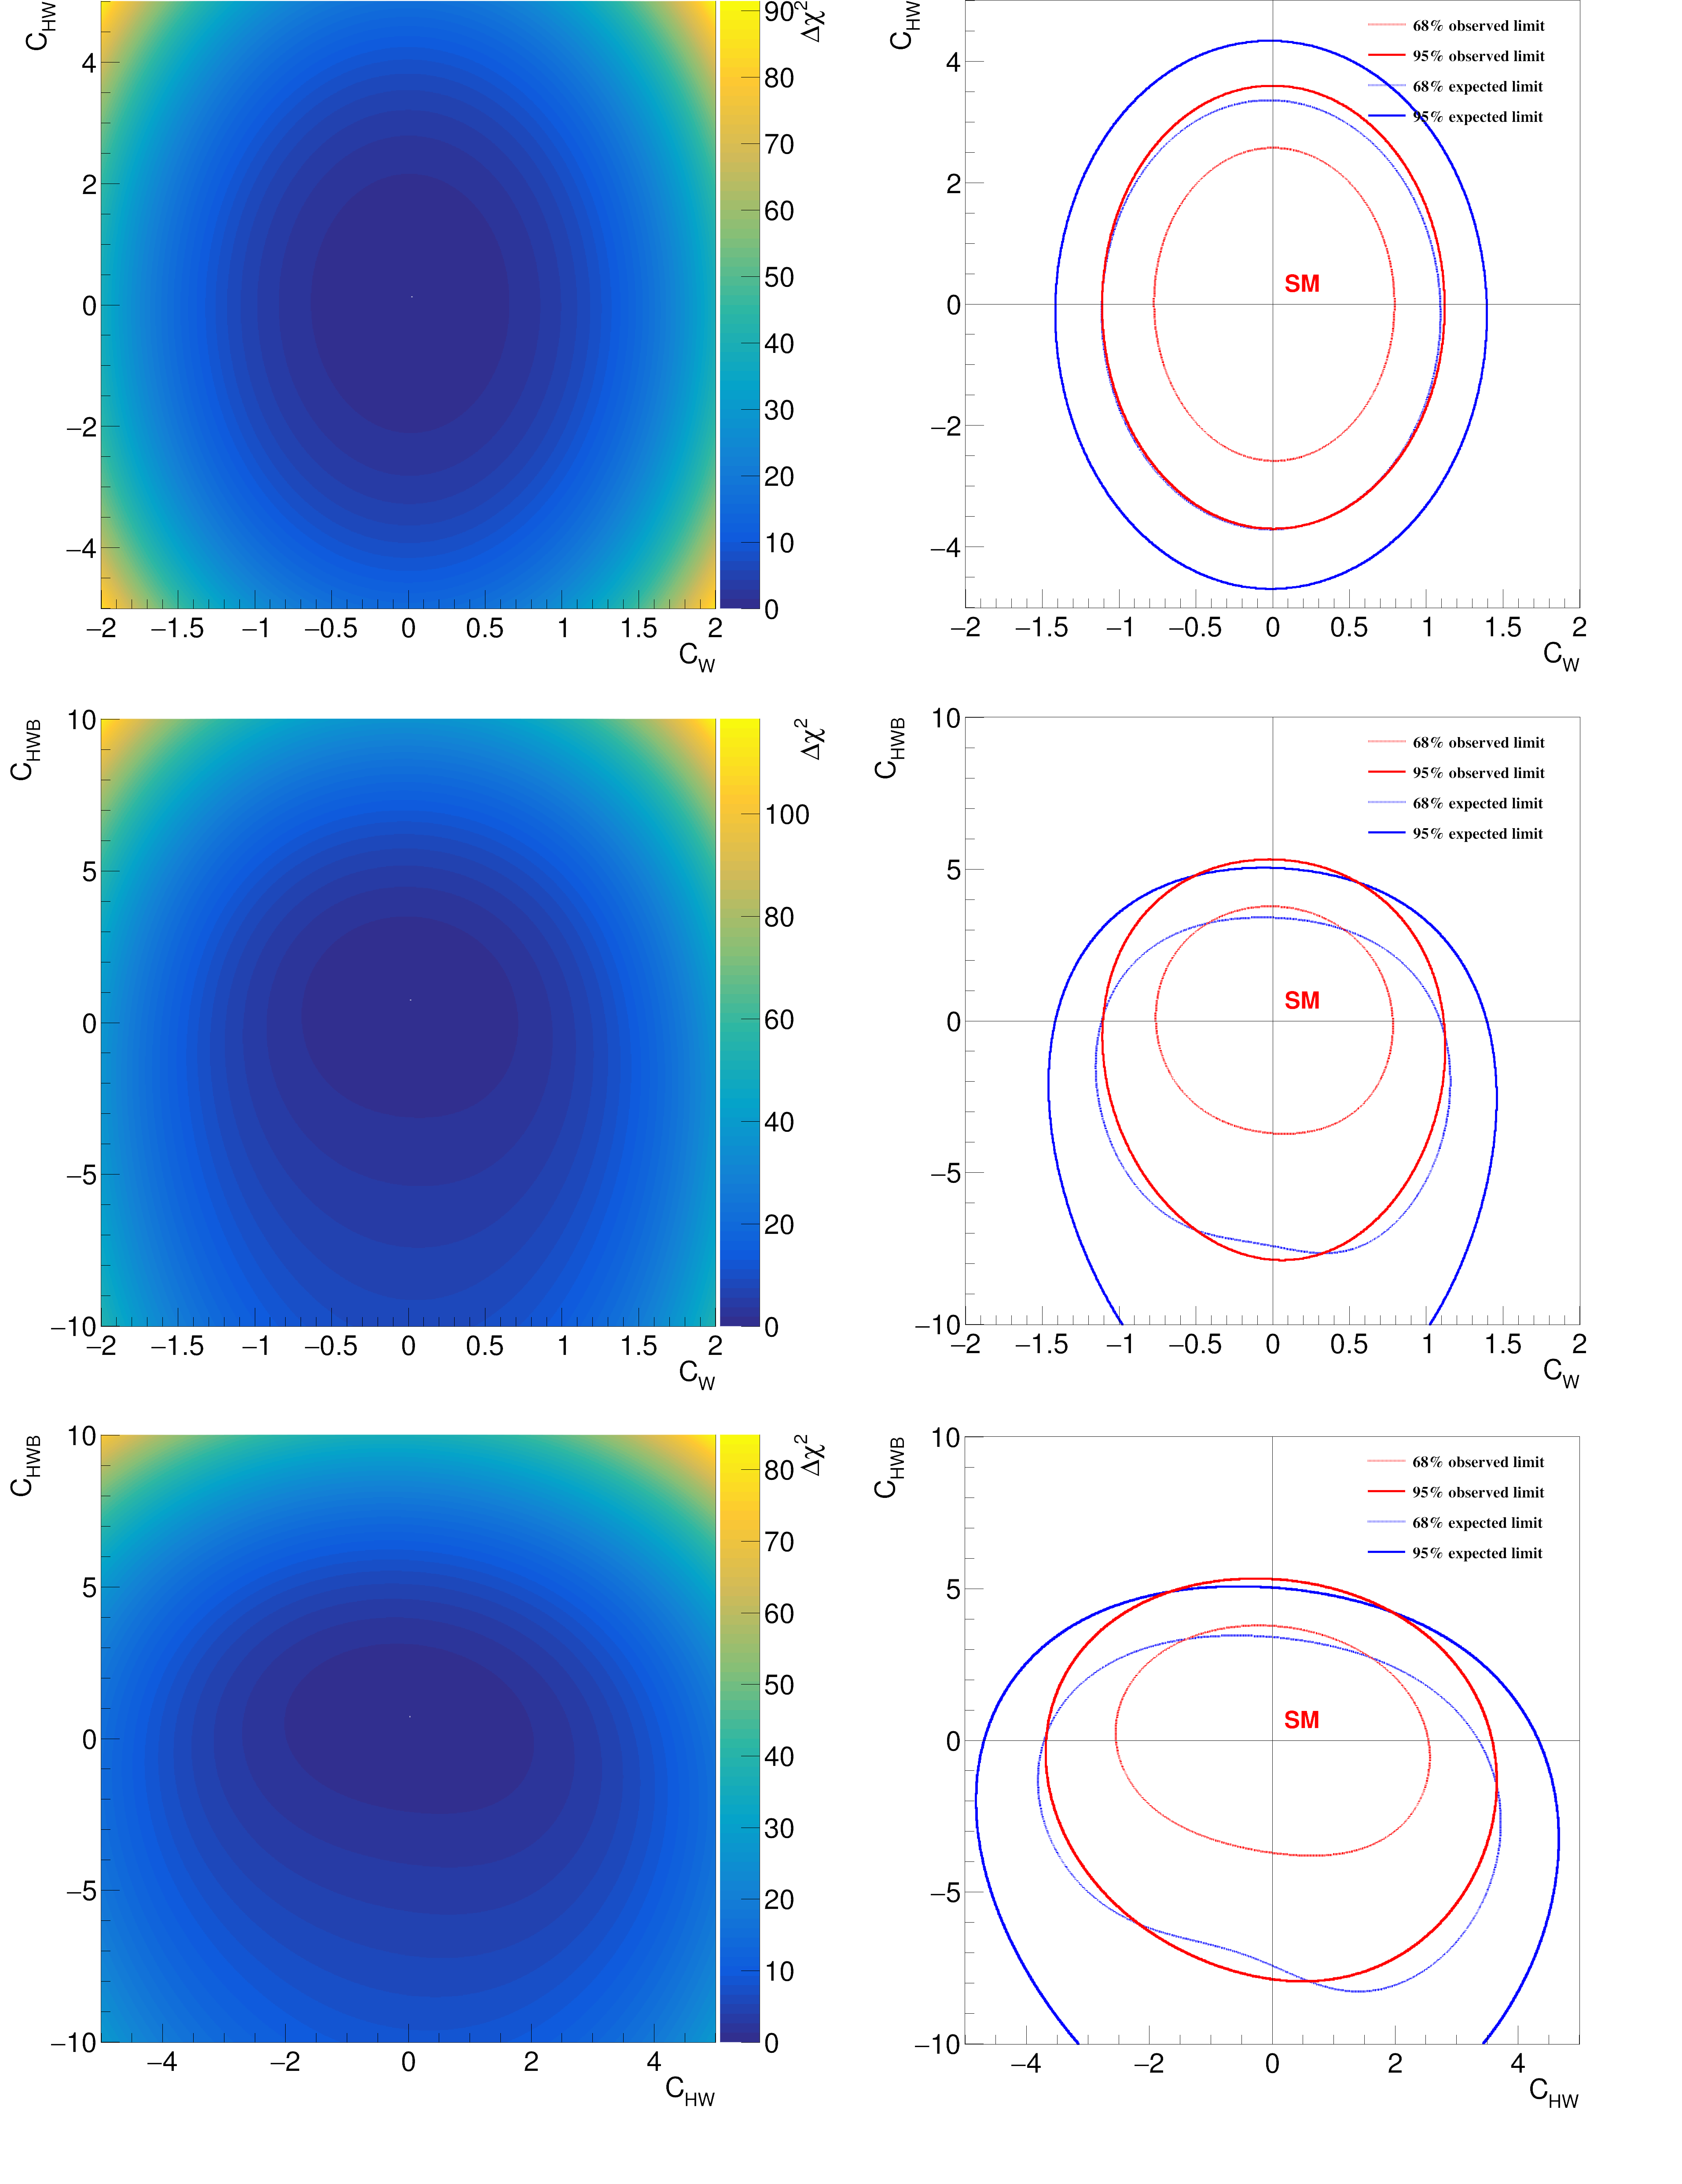
\includegraphics[scale=0.1122]{figures/limitC.png}
			\caption{\textbf{(Left)} The $\Delta\chi^2$ calculated using the $\theta_1$ distribution on the plane where 2 CP-even Wilson coefficients were scanned. 
					 \textbf{(Right)} 68\% and 95\% expected and observed limits on the 2 Wilson coefficients.
					 From top to bottom there are the $C_{HW}$ and $C_{HWB}$ plane,  $C_{W}$ and $C_{HWB}$ plane and $C_{W}$ and $C_{HW}$ plane.}
			\label{fig:LimitC}
			\end{centering}
		\end{figure}

		\begin{table}[ht!]
			\centering
			\renewcommand{\arraystretch}{1.2}
			\begin{tabularx}{\textwidth}{l X} 
			\hline\hline
			Coeff. 				& {\begin{tabularx}{0.9\textwidth}{X X X X X}		Distro.  				& 68\% obs. 		& 95\% obs.			& 68\% exp.			&  95\% exp.\end{tabularx}}	\\
			\hline
			$C_W$   			& {\begin{tabularx}{0.9\textwidth}{X X X X X}$\theta_1$			& [-0.37, 0.41]			& [-0.66, 0.68]		& [-0.64, 0.62]		& [-0.89, 0.88]  \\
															$\Delta\phi_{jj}$	& [-0.80, 0.39] 		& [-1.06, 0.82] 	& [-0.72, 0.65] 	& [-1.01, 0.94]\end{tabularx}}	\\
			\hline
			$C_{\tilde{W}}$    	& {\begin{tabularx}{0.9\textwidth}{X X X X X}$\theta_1$			& [-0.41, 0.36]			& [-0.69, 0.63] 	& [-0.64, 0.58] 	& [-0.90, 0.84] \\
															$\Delta\phi_{jj}$  	& [-0.06, 0.56]			& [-0.38, 0.81]		& [-0.31, 0.31]		& [-0.59, 0.58]\end{tabularx}}	\\
			\hline
			$C_{HW}$            & {\begin{tabularx}{0.9\textwidth}{X X X X X}$\theta_1$			& [-1.24, 1.33]			& [-2.22, 2.17]		& [-2.16, 1.83]	& [-3.01, 2.66] \\
															$\Delta\phi_{jj}$  	& [-2.78, 1.55]			& [-3.65, 2.67]		& [-2.62, 1.94]	& [-3.53, 2.85]\end{tabularx}}	\\
			\hline
			$C_{H\tilde{W}}$    & {\begin{tabularx}{0.9\textwidth}{X X X X X}$\theta_1$			& [ 0.30, 0.99]			& [-0.03, 1.33]		& [-0.32, 0.33]		& [-0.64, 0.65] \\
															$\Delta\phi_{jj}$	& [-0.03, 0.37]			& [-0.23, 0.57]		& [-0.19, 0.19]   	& [-0.37, 0.38] \end{tabularx}}	\\
			\hline
			$C_{HWB}$           & {\begin{tabularx}{0.9\textwidth}{X X X X X}$\theta_1$			& [-0.96, 1.62]		& [-2.58, 2.65]	& [-1.54, 1.28]	& [-3.55, 2.35] \\
															$\Delta\phi_{jj}$	& [-11.4, 1.06]		& [-13.1, 2.35]		& [-2.04, 1.51]   	& [-11.9, 2.72] \end{tabularx}}	\\
			\hline
			$C_{H\tilde{W}B}$   & {\begin{tabularx}{0.9\textwidth}{X X X X X}$\theta_1$			& [-2.17, 4.60]			& [-5.24, 6.68]		& [-5.52, 5.18] 	& [-7.79, 7.44] \\
															$\Delta\phi_{jj}$	& [-2.38, 4.96]			& [-5.51, 7.35]		& [-3.52, 3.58]   	& [-6.14, 6.24] \end{tabularx}}	\\
			\hline\hline
			\end{tabularx}
			\caption{The observed and expected 68\% and 95\% constraints on single Wilson coefficient calculated using the $\Delta\phi_{jj}$ and $\theta_1$ distributions. In general,
			the $\Delta\phi_{jj}$ distribution is more sensitive to the CP-odd EFT operators whereas the $\theta_1$ distribution is more sensitive to the CP-even operators.}
			\label{tab:limit}
		\end{table}
	\section{Discussion}
		\par The process of EW ZZjj with on-shell Z bosons shows good sensitivity to selected EFT operators in the fiducial region.
		Compared to the $H\rightarrow Z^{*}Z\rightarrow 4l$ process\cite{Bernlochner_2019}, constraints on operators corresponding 
		to $C_HW$, $C_{H\tilde{W}}$ and $C_{HWB}$, $C_{H\tilde{W}B}$ are tighter. The model-independent technique shows good 
		robustness and the CP-sensitive observables are proved useful.
		\par However, there are a few limitations.
		Firstly, although large sets of EFT events were generated, due to the low branching
		ratio only around 2000 events were eventually selected in the fiducial region, which can lead to rather large statistical 
		fluctuations. These uncertainties were not taken into account in the limit setting procedure.
		
		Secondly, only statistical uncertainties were considered, systematical and theoretical uncertainties in both EFT and SM 
		distributions were not taken into account. Lower sensitivities are expected if these uncertainties are being considered.
		
		Thirdly, The NDF of the $\chi_2$ distributions should be determined experimentally using large sets of pseudo-experiments, 
		however, in this analysis, they are set to 1 or 2 depending on the number of involved Wilson coefficients.

		Finally, if more than one Wilson coefficients were non-zero values, the $\Lambda^{-4}$ correction to the cross section
		should also contain the interference between these Wilson coefficients, which can only be ignored when 
		$C_1C_2/\Lambda^{-4}$ is small compared to other $\Lambda^{-4}$ contributions, in other words one of the involving 
		Wilson coefficients is small compared to the other one. These corrections was ignored regardlessly in this report.
		\par Future development of this analysis can be carried out based on these limitations, constraints on other new 
		physics models can also be easily estimated using the same technique. 

	\clearpage
	\bibliographystyle{JHEP}
	\bibliography{bibli.bib}
\end{document}
